This subsection describes the experiments that uncovers the best combination of hidden layers, neurons and epochs as well as the different strategies. Based on the above analysis of wind production influences the network will be tested with combinations of the following input parameters:

\begin{itemize}
\item Wind speed;
\item Air density;
\item Consumption;
\item Time of day;
\item Temperature;
\item Wind direction;
\item Last known production;
\item Date;
\end{itemize}

Furthermore, experiments are needed to investigate the influence of data manipulation and statistical inputs as presented in Section~\ref{sec:usingStatisticalInput}. 

\todo{DRAWING OF NETWORK}

\subsection{Experiment Series One - Selection of input parameters}
The first experiment series is an attempt to find the best constitution of network input parameters based on the analysis in Section~\ref{sec:windPowerAnalysis}. All test results can be seen in Appendix~\ref{sec:windResultsAppendix} and have been carried out naively with only normalization - relevant results will be shown here. Since the co-relation between wind production and wind speed is very significant it will always be included as a core input parameter in all test combinations.

\footnotesize
\begin{center}
\begin{longtable}{|c|c|c|c|c|c|c|c|c|c|}
\hline
\textbf{WS} & \textbf{AD} & \textbf{C} & \textbf{T} & \textbf{WD} & \textbf{L-P} & \textbf{Mo}& \textbf{ToD} & \textbf{MAE} & \textbf{Rank} \\
\hline
\endfirsthead
\multicolumn{9}{c}%
{\tablename\ \thetable\ -- \textit{Continued from previous page}} \\
\hline
\textbf{WS} & \textbf{AD} & \textbf{C} & \textbf{T} & \textbf{WD} & \textbf{L-P} & \textbf{Mo}& \textbf{ToD} & \textbf{MAE} & \textbf{Rank} \\
\hline
\endhead
\hline \multicolumn{9}{r}{\textit{Continued on next page}} \\
\endfoot
\hline
\endlastfoot
\arrayrulecolor{light-gray}
 x &  x &  x &  &  &  x &  &  x & 125.31 & \#1 \\ \hline
 x &  &  x &  &  &  x &  &  x & 128.35 & \#2 \\ \hline
 x &  x &  &  x &  x &  x &  &  x & 128.75 & \#3 \\ \hline
 x &  x &  &  &  &  x &  &  x & 130.0 & \#4 \\ \hline
 x &  x &  &  x &  &  x &  &  x & 133.38 & \#5 \\ \hline
 x &  &  &  &  &  x &  &  x & 133.99 & \#6 \\ \hline
 x &  x &  &  &  &  x &  x &  x & 134.69 & \#7 \\ \hline
 x &  x &  x &  &  &  x &  x &  x & 134.73 & \#8 \\ \hline
 x &  x &  &  &  x &  x &  &  x & 134.79 & \#9 \\ \hline
 x &  &  x &  x &  &  x &  &  x & 136.2 & \#10 \\ \hline
 . & . & . & . &  .  & . &  . & . & . & . \\ 
 . & . & . & . &  .  & . &  . & . & . & . \\ 
 . & . & . & . &  .  & . &  . & . & . & .\\ \hline
 x &  &  &  x &  x &  &  &  x & 160.86 & \#55 \\ \hline
 x &  x &  x &  x &  x &  &  &  x & 162.45 & \#56 \\ \hline
 x &  x &  x &  x &  x &  &  x &  x & 164.28 & \#57 \\ \hline
 x &  &  &  x &  x &  x &  x &  x & 165.25 & \#58 \\ \hline
 x &  &  &  &  &  x &  x &  x & 166.25 & \#59 \\ \hline
 x &  x &  &  &  &  &  &  x & 167.38 & \#60 \\ \hline
 x &  &  x &  x &  x &  x &  x &  x & 169.88 & \#61 \\ \hline
 x &  &  &  x &  &  x &  x &  x & 171.49 & \#62 \\ \hline
 x &  x &  &  &  x &  x &  x &  x & 171.7 & \#63 \\ \hline
 x &  &  x &  x &  x &  &  x &  x & 175.32 & \#64 \\ \hline
\caption{Wind Production Input Parameter Test Top and bottom 10. It is based on 3 month of historical data and 200 epochs. It is an average of the prediction over 8000 hours}
\end{longtable}
\label{table:windProdInputParamsTop10}
\end{center}
\normalsize

All results from the first experiment can be seen in Appendix~\ref{sec:simpleInputTest}. The results vary from the best MAE at 123,29 to the worst being 175,32. Top and bottom 10 is shown in Table~\ref{table:windProdInputParamsTop10} indicated by rank. The experiment clearly show the importance of air density, time of day and last production. This correspond well with the analysis in Section~\ref{sec:windPowerAnalysis} where the relationship between wind production and the parameters are established to be significant. Especially the analysis concerning the importance of wind production development and time of day is  seen in the experiments. The production does not differ much from one hour to the next which is reflected in the last known production input parameter --- more sophisticated attempts with statistic will be in experiments to come. What comes as a surprise is the under representation of consumption in top 10 because the analysis showed a good co-relation. It can be explained by a bad co-relation between consumption and some of the other input parameters that makes more noise and influence the prediction badly. The analysis section also discussed the substitution of temperature with consumption --- this is obviously not the best solution when looking at rank \#2 and \#6 where the substitution results in a decrease in MAE.\todo{discuss wind direction}. What is obvious from the experiment is the impact of month as input parameter and how it in general does not help the prediction. What comes to mind is the historical data used for testing. Month represents the seasonal perspective and is suppose to find the relation between months in general and the production. Since the historical data used for prediction is only 3 months, it does not capture how months in general influenced the production in the past year. A possible solution to obtain the seasonality aspect is presented in\cite{pjmForecast} where the Neural Network is trained with 45 days from before the day to be predicted, and 45 days before and after in the previous year. By using this approach the month parameter will reflect the influence of the months around you from the last year. This needs validation in an experiment for itself. The experiment results can be seen in Table~\ref{table:seasonalWindProdInputParamsTop10}. What is clear is the immediate decrease in MAE. This can be explained by the increase data in the training set which makes it harder for the ANN to generalize. According to\cite{1} too large training sets should be avoided because it has a tendency to be overtrained. The possible benefits from including the seasonal aspect when predicting wind production can not make up for the loss in accuracy by the increase in the size of training data. To completely eliminate any doubts about the decrease in accuracy when using season, another test on an entire year has been conducted. Results can be seen in Table~\ref{table:seasonWindProdInputParamsTop2WholeYear}. The two results are using the same input parameters as \#7 and \#8 in Table~\ref{table:windProdInputParamsTop10} and the MAE is around 10 worse in both cases. The usage of only 3 months in the dataset can be argued to contain the seasonal aspect for the hours to predict. The three months in the set will reflect the current season that you are in and therefore more data will only create more noise. The month parameter will not say anything about the past year but only the months it has already seen. It will also include the transitions between the seasons instead of putting the seasons into boxes, e.g. when moving into summer from winter, the month parameter over an entire year would immediately put it into the summer box. It needs to be made clear that it is only worsened with 10 in average and it is only one input parameter of the entire network. The above discussion clearly illustrates that the small data itself contains the seasonality itself because the network trains and generalizes only upon the current season. For this reason the month parameter is not needed in this case which is also clear from the Table~\ref{table:windProdInputParamsTop10} where top 6 is without month and almost 10 better. \todo{argument and compare curves from 2012 and 2011}. 

In experiments concerning prediction of wind production the month input parameter will be left out.  

\footnotesize
\begin{center}
\begin{longtable}{|c|c|c|c|c|c|c|c|c|c|}
\hline
\textbf{WS} & \textbf{AD} & \textbf{C} & \textbf{T} & \textbf{WD} & \textbf{L-P} & \textbf{Mo}& \textbf{ToD} & \textbf{MAE} & \textbf{Rank} \\
\hline
\endfirsthead
\multicolumn{9}{c}%
{\tablename\ \thetable\ -- \textit{Continued from previous page}} \\
\hline
\textbf{WS} & \textbf{AD} & \textbf{C} & \textbf{T} & \textbf{WD} & \textbf{L-P} & \textbf{Mo}& \textbf{ToD} & \textbf{MAE} & \textbf{Rank} \\
\hline
\endhead
\hline \multicolumn{9}{r}{\textit{Continued on next page}} \\
\endfoot
\hline
\endlastfoot
\arrayrulecolor{light-gray}
 x &  x &  &  &  &  x &  &  x & 139.38 & \#1 \\ \hline
 x &  x &  x &  &  &  x &  &  x & 139.89 & \#2 \\ \hline
 x &  x &  x &  x &  x &  x &  &  x & 140.09 & \#3 \\ \hline
 x &  x &  &  x &  &  x &  &  x & 140.59 & \#4 \\ \hline
 x &  &  x &  &  &  x &  &  x & 141.66 & \#5 \\ \hline
 x &  x &  &  &  x &  x &  &  x & 142.72 & \#6 \\ \hline
 x &  &  x &  &  &  x &  x &  x & 142.77 & \#7 \\ \hline
 x &  x &  &  &  &  &  &  x & 144.08 & \#8 \\ \hline
 x &  &  &  &  x &  x &  &  x & 144.35 & \#9 \\ \hline
 x &  x &  x &  &  x &  &  &  x & 144.47 & \#10 \\ \hline
\caption{Top 10 seasonal wind production test. It is based on 3 month of historical data and one month after from the previous year. It is run with 200 epochs and predicts 8000 hours in 2012}
\end{longtable}
\label{table:seasonalWindProdInputParamsTop10}
\end{center}
\normalsize



\todo{trend discussion in relation to why seasonal impl is better on small dataset}.

\footnotesize
\begin{center}
\begin{longtable}{|c|c|c|c|c|c|c|c|c|c|}
\hline
\textbf{WS} & \textbf{AD} & \textbf{C} & \textbf{T} & \textbf{WD} & \textbf{L-P} & \textbf{Mo}& \textbf{ToD} & \textbf{MAE} & \textbf{Rank} \\
\hline
\endfirsthead
\multicolumn{9}{c}%
{\tablename\ \thetable\ -- \textit{Continued from previous page}} \\
\hline
\textbf{WS} & \textbf{AD} & \textbf{C} & \textbf{T} & \textbf{WD} & \textbf{L-P} & \textbf{Mo}& \textbf{ToD} & \textbf{MAE} & \textbf{Rank} \\
\hline
\endhead
\hline \multicolumn{9}{r}{\textit{Continued on next page}} \\
\endfoot
\hline
\endlastfoot
\arrayrulecolor{light-gray}
 x &  x &  x &  &  &  x &  x &  x & 143.23 & \#1 \\ \hline
 x &  x &  &  &  &  x &  x &  x & 147.98 & \#2 \\ \hline
\caption{Seasonal wind production test based on an entire year. It is run with 200 epochs and predicts 8000 hours in 2012}
\end{longtable}
\label{table:seasonWindProdInputParamsTop2WholeYear}
\end{center}
\normalsize
\todo{see appendix}


The three best ranked combination of parameters will be the basis for all coming experiments. The prediction for the first 175 hours can be seen in Figure~\ref{fig:bestInputParameterPrediction}. It can be seen that the prediction follows the trend of the actual wind production. The obvious challenge is that the prediction takes time to identify shifting trend --- either it identifies it before happens or after it happened. From hour 25-50 it is way behind the actual slope. It can also be seen around hour 100-110 that it significantly overshoots and in 110-150 undershoots its target before actually identifying the shift. The statistical approach described in Section~\ref{sec:usingStatisticalInput} can possible help in these cases by taking current trend into consideration. Experiments will take up this approach for comparison.  

\begin{figure}[H]
\centering
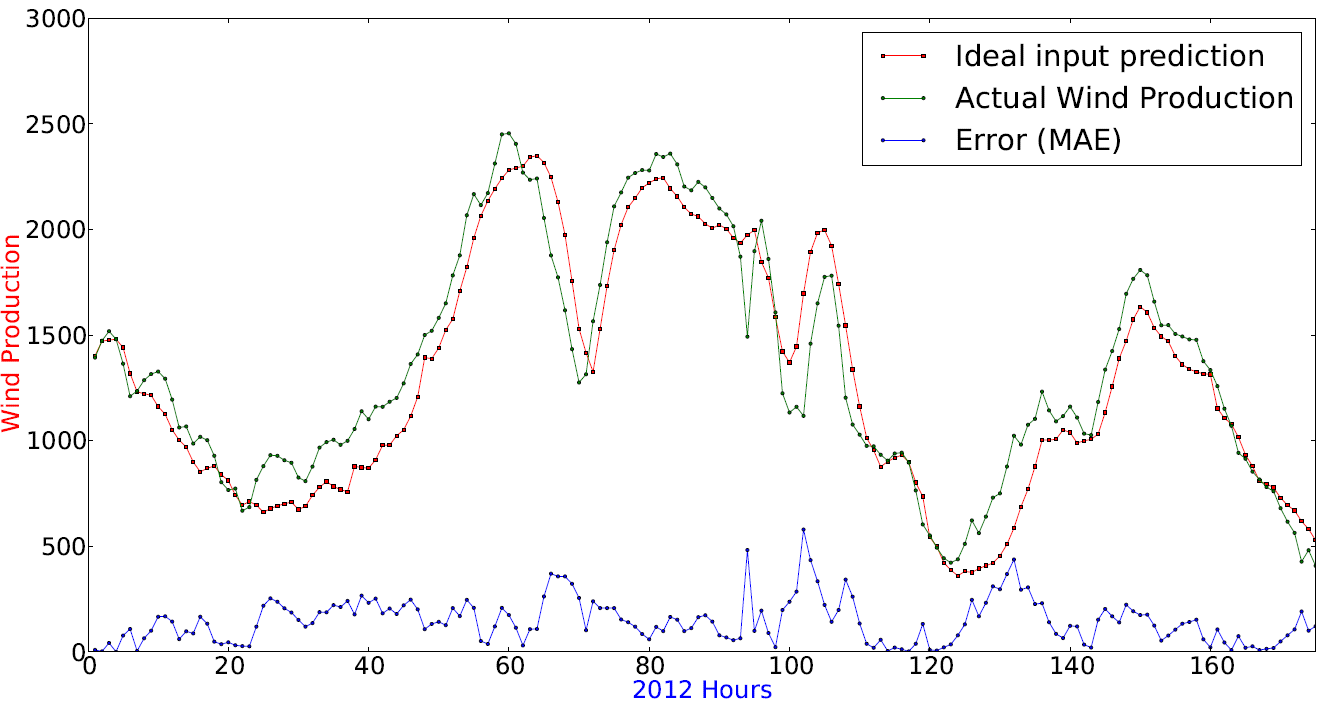
\includegraphics[width=0.99\linewidth]{billeder/bestInputParameterPrediction.png}
\caption{Wind production prediction for 175 hours in 2012}
\label{fig:bestInputParameterPrediction}
\end{figure}   

The experiments to come will be based on input combinations from the top 3 from Table~\ref{table:windProdInputParamsTop10}. The inputs are:
\begin{itemize}
\item Wind speed;
\item Air density;
\item Consumption;
\item Wind Direction;
\item Temperature;
\item Last known production;
\item Time of day;
\end{itemize}

\subsection{Experiment Two - Data Manipulation}
Trimming is only an issue if irregularities exist\todo{use curves to illustrate that it is not necessary here}. The purpose of the experiments in series two is to turn inputs into a matrix whenever possible. As described in Section~\ref{sec:Matrix} one input parameter is split into one input parameter for all of its possible values --- it makes sense because each input parameter has a weight that is adjusting itself according to the error as illustrated in Section~\ref{sec:annSection}. This is of course only an option if all values are known in advance and of a manageable size. When considering wind production forecasting this is valid for hours of the day, month and wind speed. Wind speeds are represented  by 41 different speeds in our data set. Instead of having only one input to represent each of the values, we can have 41 inputs for every single one of them. The purpose is to have a weight that tells exactly how much the specific input parameter in general influence the wind production to predict. Whenever a specific value is inserted it will be indicated with 1 and the rest of the matrix with 0. The network will then be adjusting a weight for the different entrances in the matrix whenever they are seen. What can become a problem is if some values does not exist or are under-represented which will cause that specific value to be under-expressed and not able to cover unseen data because the weight has only been adjusted a few times or not at all. In theory the matrix manipulation makes the most sense when all values to some degree are equally distributed so that every input in the matrix can express all values equally. Consider the case where wind speed 5 is not represented in the training dataset but is in the prediction data set, the network then won't have any clue how to relate to 5 when using the matrix implementation. In this case it makes sense to use one input parameter as representation because one weight have been adjusted to all the other values and illustrates how they in general influence the wind production. With that information contained in the weight it can also express 5 when the two are multiplied. Hours of the day and months are of course equally distributed. 

\footnotesize
\begin{center}
\begin{longtable}{|c|c|c|c|c|c|c|c|c|c|}
\hline
\textbf{WS} & \textbf{AD} & \textbf{C} & \textbf{T} & \textbf{WD} & \textbf{L-P} & \textbf{Mo}& \textbf{ToD} & \textbf{MAE} & \textbf{Rank} \\
\hline
\endfirsthead
\multicolumn{10}{c}%
{\tablename\ \thetable\ -- \textit{Continued from previous page}} \\
\hline
\textbf{WS} & \textbf{AD} & \textbf{C} & \textbf{T} & \textbf{WD} & \textbf{L-P} & \textbf{Mo}& \textbf{ToD} & \textbf{MAE} & \textbf{Rank} \\
\hline
\endhead
\hline \multicolumn{10}{r}{\textit{Continued on next page}} \\
\endfoot
\hline
\endlastfoot
\arrayrulecolor{light-gray}
 \x &  &  \x &  &  &  \x &  &  \x (m) &120.17 & \#1 \\ \hline
 \x &  \x &  &  \x &  &  \x &  &  \x (m) &127.82 & \#2 \\ \hline
 \x &  \x &  \x &  &  &  \x &  &  \x (m) &131.61 & \#3 \\ \hline
 \x &  \x &  \x &  &  &  \x &  &  \x & 135.54 & \#4 \\ \hline
 \x (m) & \x &  \x &  &  &  \x &  &  \x & 138.08 & \#5 \\ \hline
 \x (m) & &  \x &  &  &  \x &  &  \x & 139.99 & \#6 \\ \hline
 \x &  \x &  &  \x &  &  \x &  &  \x & 141.5 & \#7 \\ \hline
 \x &  &  \x &  &  &  \x &  &  \x & 142.7 & \#8 \\ \hline
 \x (m) & \x &  &  \x &  &  \x &  &  \x & 144.46 & \#9 \\ \hline
 \x (m) & &  \x &  &  &  \x &  &  \x (m) &146.6 & \#10 \\ \hline
 \x (m) & \x &  &  \x &  &  \x &  &  \x (m) &167.85 & \#11 \\ \hline
 \x (m) & \x &  \x &  &  &  \x &  &  \x (m) &188.37 & \#12 \\ \hline
\caption{Wind Production Input Parameter Test Top 10}
\end{longtable}
\label{table:windProdInputParamsTop10}
\end{center}
\normalsize
\todo{see appendix}

\todo{discuss how matrix both influence indirectly and directly influence the prediction. Both pros and cons. The point is that a new month will not be influenced by the month before in terms of the weight. It will have its own. You remove responsibility from the other weights, they do not have to incorporate fx. how the month influence, they can focus only on wind speed and how it relates to the output}

\subsection{Experiment Three - Statistical Inputs}
Statistics. This subsection is experimenting with the concepts described in Section~\ref{sec:usingStatisticalInput}.

\todo{also different size of dataset}

\footnotesize
\begin{center}
\begin{longtable}{|c|c|}
\hline
\textbf{Hours} & \textbf{MAE} \\
\hline
\endfirsthead
\multicolumn{2}{c}%
{\tablename\ \thetable\ -- \textit{Continued from previous page}} \\
\hline
\textbf{Hours} & \textbf{MAE} \\
\hline
\endhead
\hline \multicolumn{2}{r}{\textit{Continued on next page}} \\
\endfoot
\hline
\endlastfoot
\arrayrulecolor{light-gray}
20 & 118,15 \\ \hline
8 & 119,58 \\ \hline
12 & 121,54 \\ \hline
4 & 122,51  \\ \hline
16 & 123,87 \\ \hline
24 & 124,89 \\ \hline
6 & 129,32 \\ \hline
2 & 137,55 \\ \hline
\caption{Prediction With Historical Volatility and different hours}
\end{longtable}
\label{table:historicalVoltalityHours}
\end{center}
\normalsize

\begin{center}
\begin{longtable}{|c|c|}
\hline
\textbf{Hours} & \textbf{MAE} \\
\hline
\endfirsthead
\multicolumn{2}{c}%
{\tablename\ \thetable\ -- \textit{Continued from previous page}} \\
\hline
\textbf{Hours} & \textbf{MAE}\\
\hline
\endhead
\hline \multicolumn{2}{r}{\textit{Continued on next page}} \\
\endfoot
\hline
\endlastfoot
\arrayrulecolor{light-gray}
2 & 114,71 \\ \hline
8 & 116,09 \\ \hline
12 & 117,33\\ \hline
4 & 117,49  \\ \hline
16& 118,09  \\ \hline
20 & 119,35 \\ \hline
6 & 120,64 \\ \hline
24 & 121,67 \\ \hline
\caption{Prediction With Skewness and different hours}
\end{longtable}
\label{table:skewnessHours}
\end{center}
\normalsize


\begin{center}
\begin{longtable}{|c|c|}
\hline
\textbf{Hours} & \textbf{MAE} \\
\hline
\endfirsthead
\multicolumn{2}{c}%
{\tablename\ \thetable\ -- \textit{Continued from previous page}} \\
\hline
\textbf{Hours} & \textbf{MAE} \\
\hline
\endhead
\hline \multicolumn{2}{r}{\textit{Continued on next page}} \\
\endfoot
\hline
\endlastfoot
\arrayrulecolor{light-gray}
24 & 119,73 \\ \hline
12 & 126,62 \\ \hline
20 & 126,84 \\ \hline
16 & 129,87 \\ \hline
6 & 135,56 \\ \hline
4 & 140,18 \\ \hline
8 & 141,36 \\ \hline
2 & 146,13 \\ \hline
\caption{Curve Analysis on different hours}
\end{longtable}
\label{table:curveAnalysisHours}
\end{center}
\normalsize

\begin{center}
\begin{longtable}{|c|c|}
\hline
\textbf{Hours} & \textbf{MAE} \\
\hline
\endfirsthead
\multicolumn{2}{c}%
{\tablename\ \thetable\ -- \textit{Continued from previous page}} \\
\hline
\textbf{Hours} & \textbf{MAE} \\
\hline
\endhead
\hline \multicolumn{2}{r}{\textit{Continued on next page}} \\
\endfoot
\hline
\endlastfoot
\arrayrulecolor{light-gray}
Skewness & 114,71 \\ \hline
Volatility & 118,15 \\ \hline
Scatter & 118,61 \\ \hline
Curve Analysis & 119,73 \\ \hline
\caption{Comparison of the approaches}
\end{longtable}
\label{table:comparisonStatistics}
\end{center}
\normalsize

\todo{say something clever about them}.
Also tried scatter as presented~\cite{singhal2011electricity}. This achieved a MAE of 118.61. A combination of the approaches is illustrated in Table~\ref{table:idealCombination}.

\begin{center}
\begin{longtable}{|c|c|c|}
\hline
\textbf{Hours} & \textbf{MAE} & \textbf{Rank} \\
\hline
\endfirsthead
\multicolumn{3}{c}%
{\tablename\ \thetable\ -- \textit{Continued from previous page}} \\
\hline
\textbf{Hours} & \textbf{MAE} & \textbf{Rank} \\
\hline
\endhead
\hline \multicolumn{3}{r}{\textit{Continued on next page}} \\
\endfoot
\hline
\endlastfoot
\arrayrulecolor{light-gray}
2 & 114.71 & \#1 \\ \hline
\caption{Ideal combination}
\end{longtable}
\label{table:idealCombination}
\end{center}
\normalsize






\todo{better with or without trimming?}


\todo{do 1-12-24 step ahead to show the "carry-with"-error} 


\subsection{Experiment Three - Prediction Strategies}

\subsection{Experiment Four - Black Box Optimization}
Statistics


\subsection{Experiment Five - Performance Optimization}
The impact of different Layers/Neurons/Epochs combinations is huge and the results is shown here.

\begin{table}[H]
\centering  % used for centering table
\begin{tabular}{c c c c c} % centered columns (3 columns)
ANN Type & Epochs & MAE & MPE & Rank \\ [0.5ex] % inserts table 
%heading
\hline                  % inserts single horizontal line
ANN & 500 & 0 & 0 & 0 \\ % inserting body of the table
ANN & 1000 & 0 & 0 & 0 \\
ANN & 2000 & 0 & 0 & 0 \\
ANN & 2500 & 0 & 0 & 0 \\ [1ex] % [1ex] adds vertical space
\hline %inserts single line
\end{tabular}
\caption{Table showing the performance of different data manipulation approaches.} % title of Table
\label{table:performanceOpti} % is used to refer this table in the text
\end{table} 
